\chapter*{Chengdu, Emeishan et Leshan\markboth{Chengdu, Emeishan et Leshan}{}}
\section*{8 octobre 2015}
Chengdu est une immense ville de plusieurs millions d'habitants.

 Place centrale avec une statue de Mao.
\begin{center} 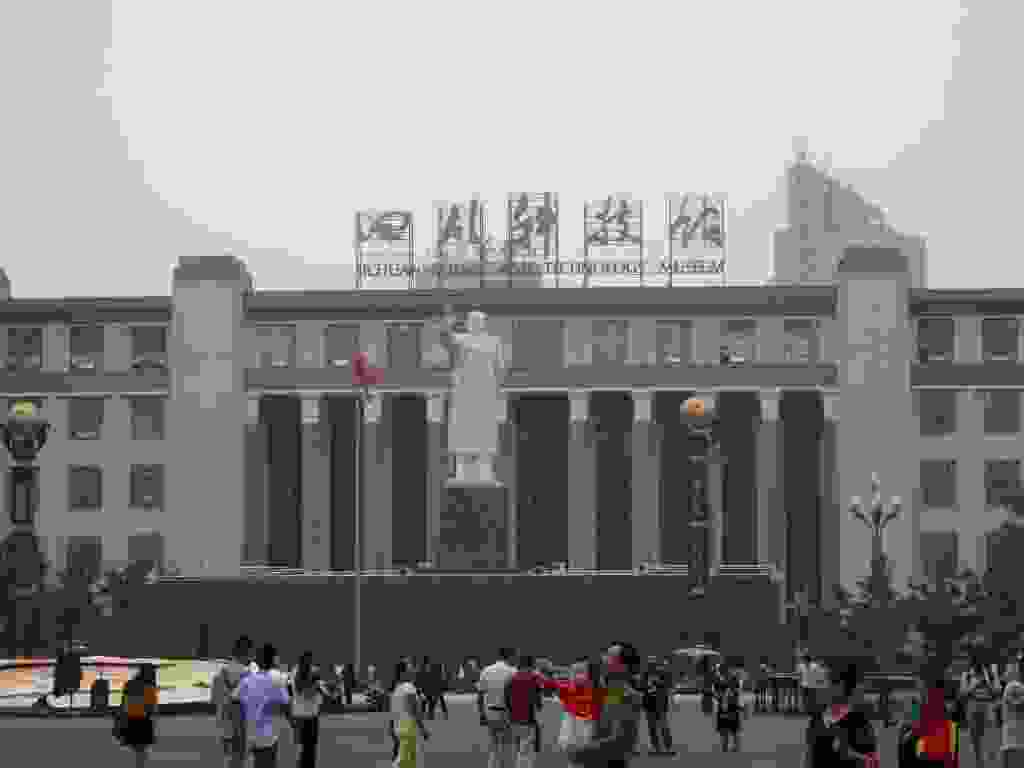
\includegraphics[width=\mywidth]{../wp-content/uploads/2015/09/wpid-p9227084-1024x768.jpg} \end{center}
\begin{center} 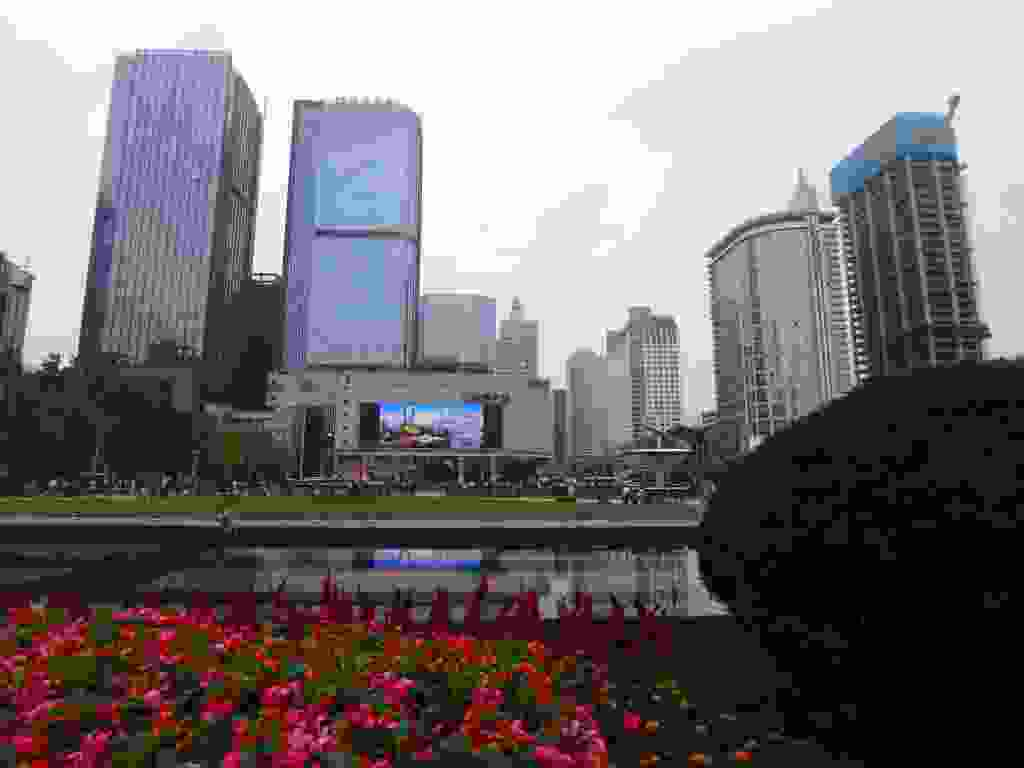
\includegraphics[width=\mywidth]{../wp-content/uploads/2015/09/wpid-p9227086-1024x768.jpg} \end{center}

 People's Park, toujours des activités variées. 
\begin{center} 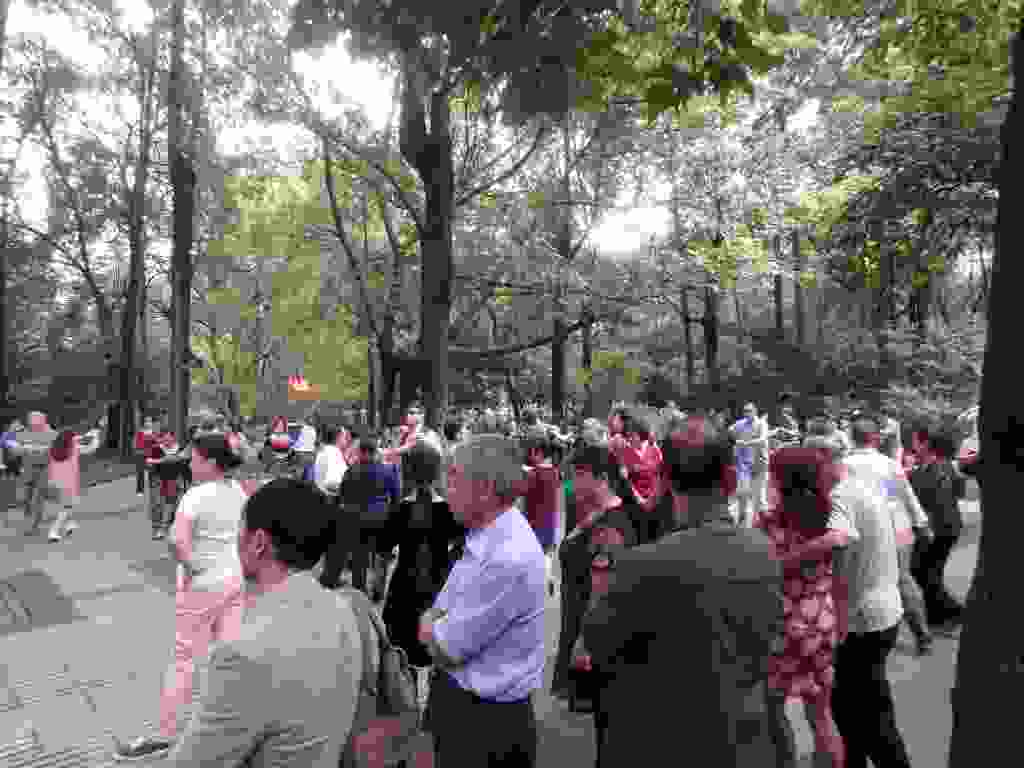
\includegraphics[width=\mywidth]{../wp-content/uploads/2015/09/wpid-p9227076-1024x768.jpg} \end{center}
\begin{center} 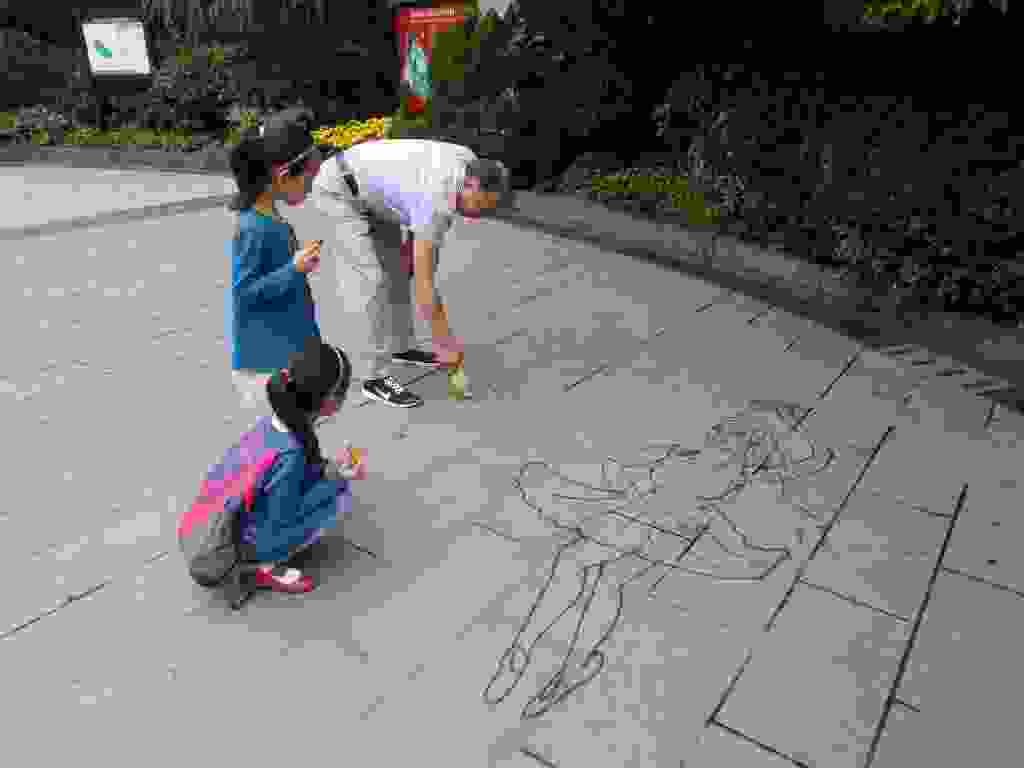
\includegraphics[width=\mywidth]{../wp-content/uploads/2015/09/wpid-p9227083-1024x768.jpg} \end{center}
\begin{center} 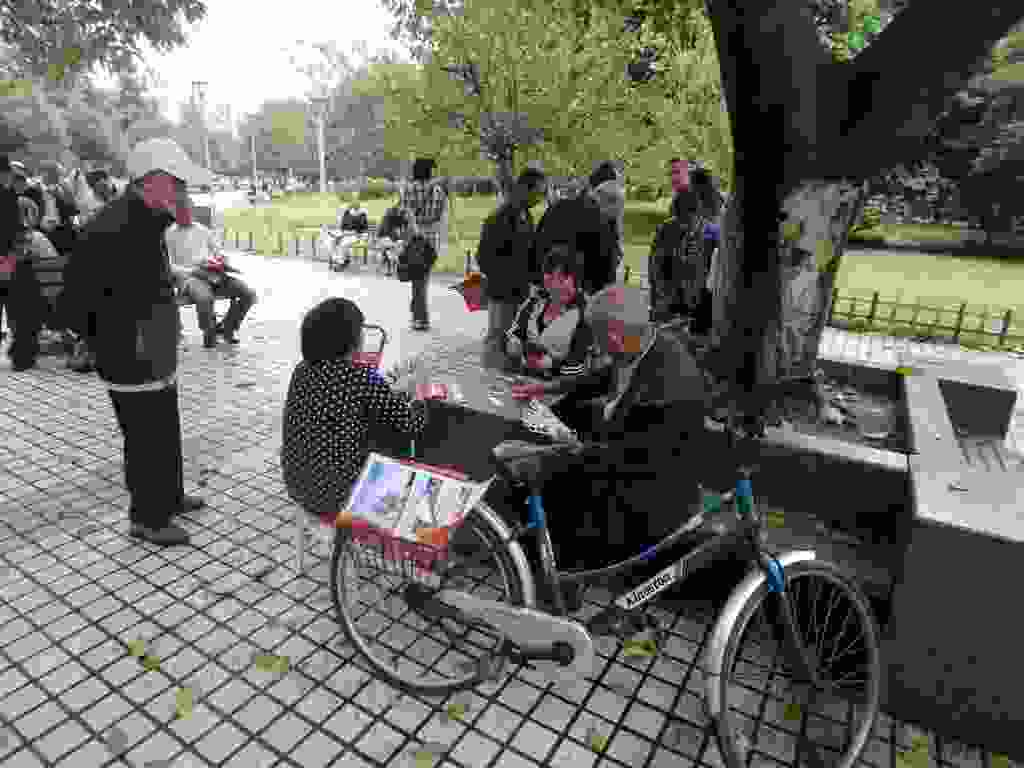
\includegraphics[width=\mywidth]{../wp-content/uploads/2015/10/wpid-p9270005-1024x768.jpg} \end{center}

\pagebreak
 Dans une allée, des parents déposent des annonces pour marier leur fille, une seule était en anglais : 
\begin{center} 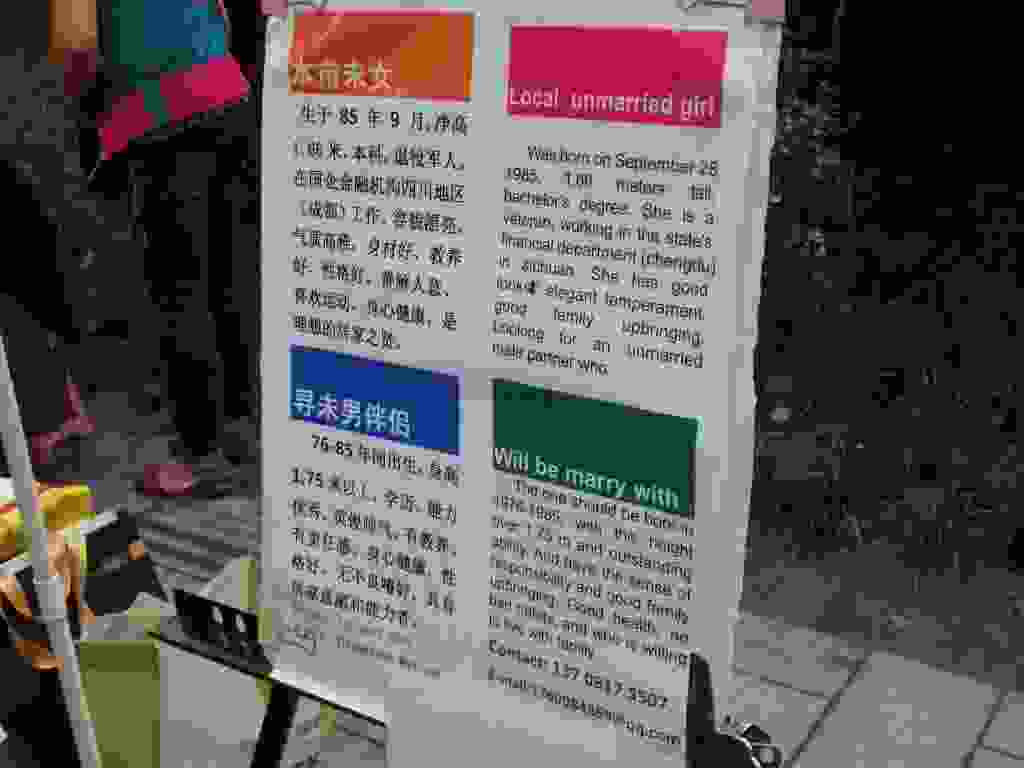
\includegraphics[width=\mywidth]{../wp-content/uploads/2015/09/wpid-p9227079-1024x768.jpg} \end{center}

 Monastère bouddhiste de Wenshu. 
\begin{center} 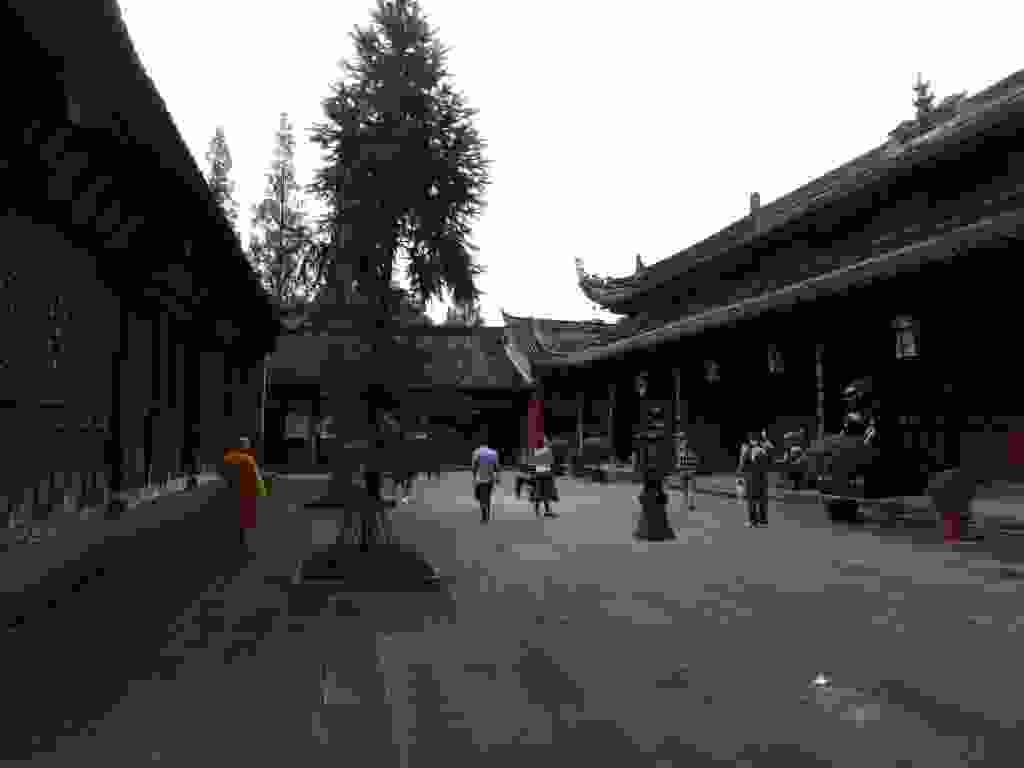
\includegraphics[width=\mywidth]{../wp-content/uploads/2015/10/wpid-p92270651-1024x768.jpg} \end{center}
\begin{center} 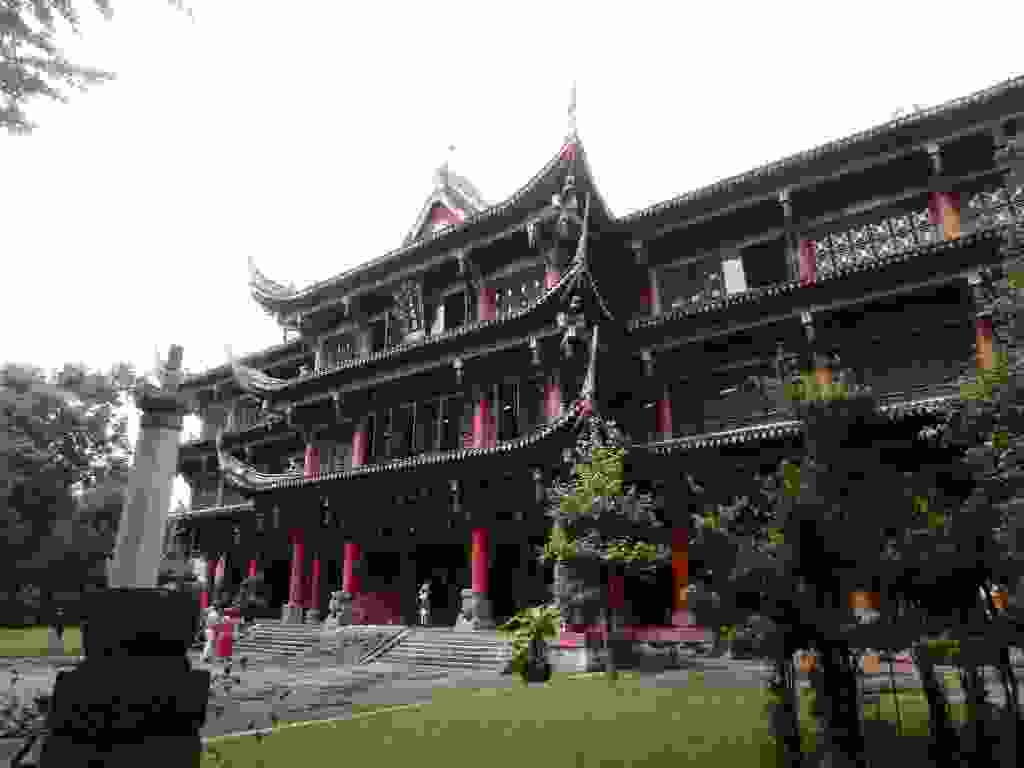
\includegraphics[width=\mywidth]{../wp-content/uploads/2015/09/wpid-p9227068-1024x768.jpg} \end{center}
\begin{center} 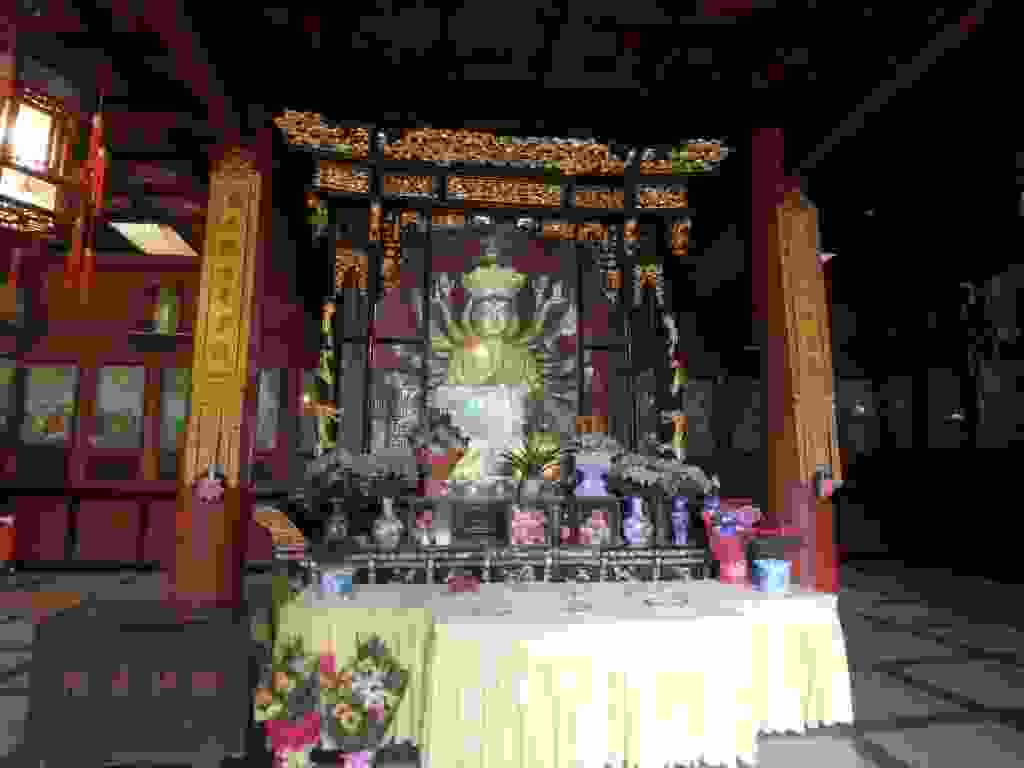
\includegraphics[width=\mywidth]{../wp-content/uploads/2015/09/wpid-p9227066-1024x768.jpg} \end{center}

\pagebreak
 Dans l'hostel où je suis à Chengdu, je rencontre Fred et Brigitte, cyclistes suisses qui roulent depuis 1 an et demi, ils ont traversé toute l'Europe puis l'Asie centrale avant d'arriver en Chine. Ils voyagent depuis 1 semaine avec Jet, chinois. 
\begin{center} 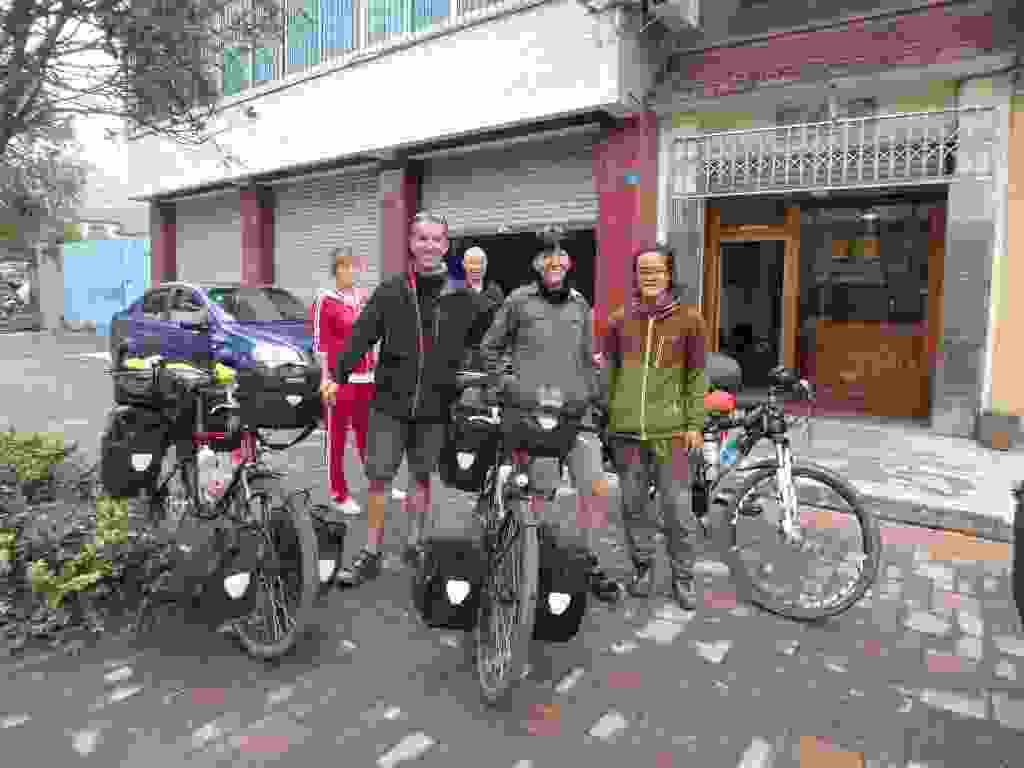
\includegraphics[width=\mywidth]{../wp-content/uploads/2015/09/wpid-p92070201-1024x768.jpg} \end{center}

 Comme ils vont vers le Sud, je me joins à eux pour quelques jours. 
\begin{center} 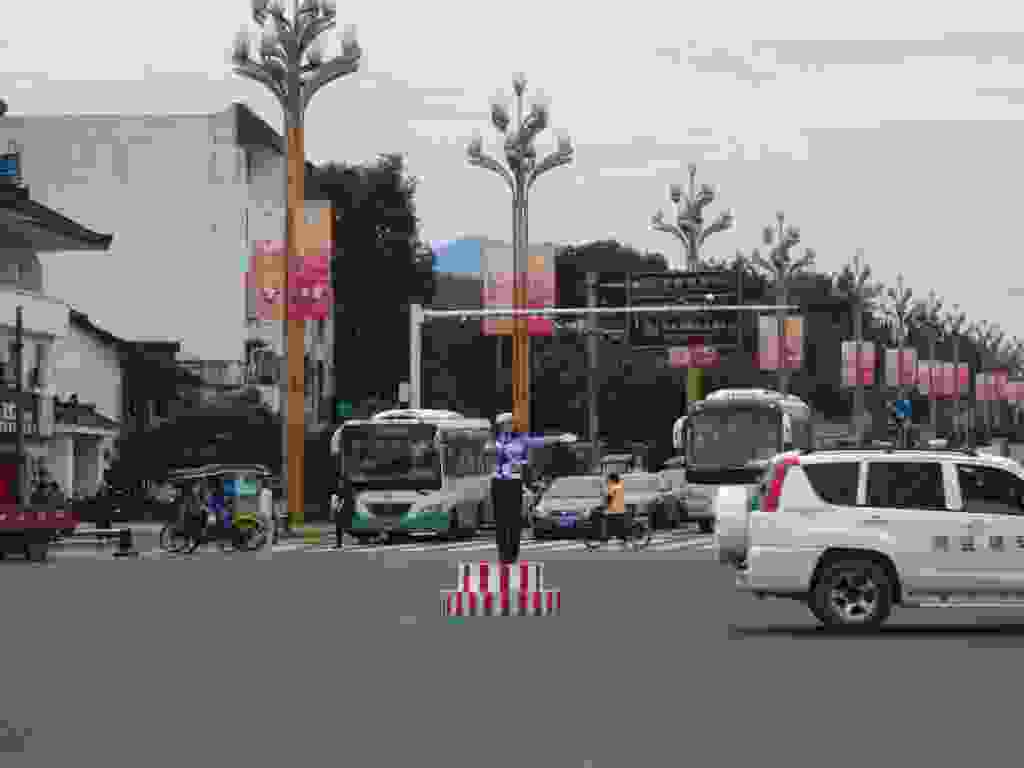
\includegraphics[width=\mywidth]{../wp-content/uploads/2015/10/wpid-p9257115-1024x768.jpg} \end{center}

\pagebreak
 Sortie de la ville, on n'est pas perdu pour faire les courses. 
\begin{center} 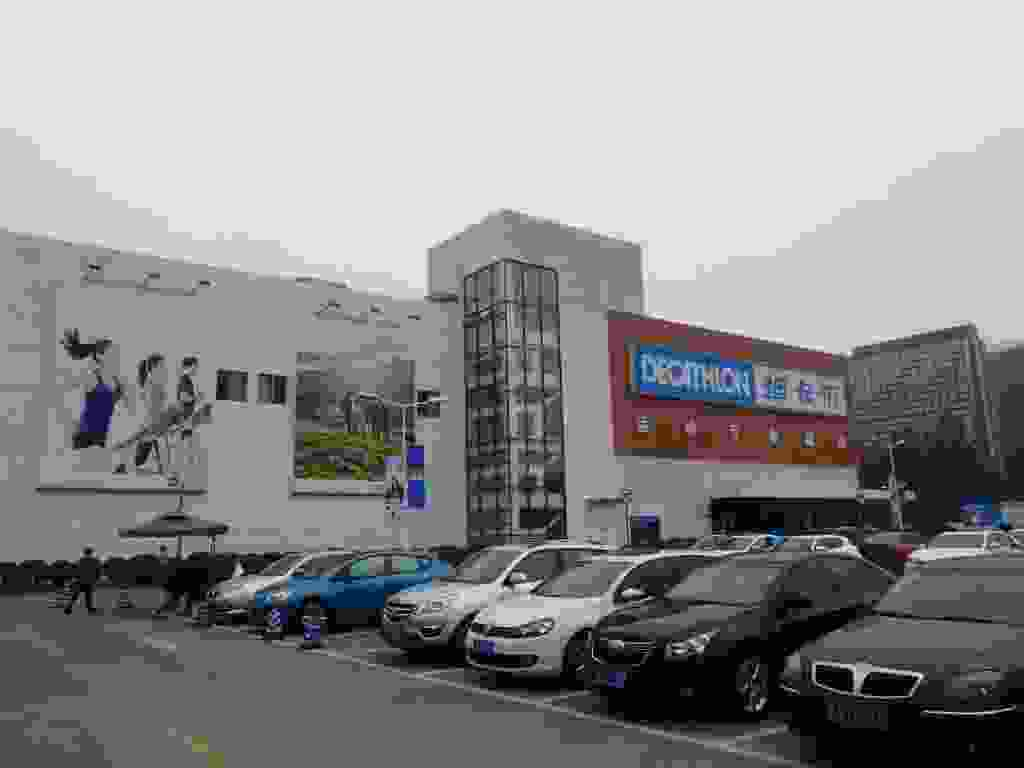
\includegraphics[width=\mywidth]{../wp-content/uploads/2015/09/wpid-p9237090-1024x768.jpg} \end{center}
\begin{center} 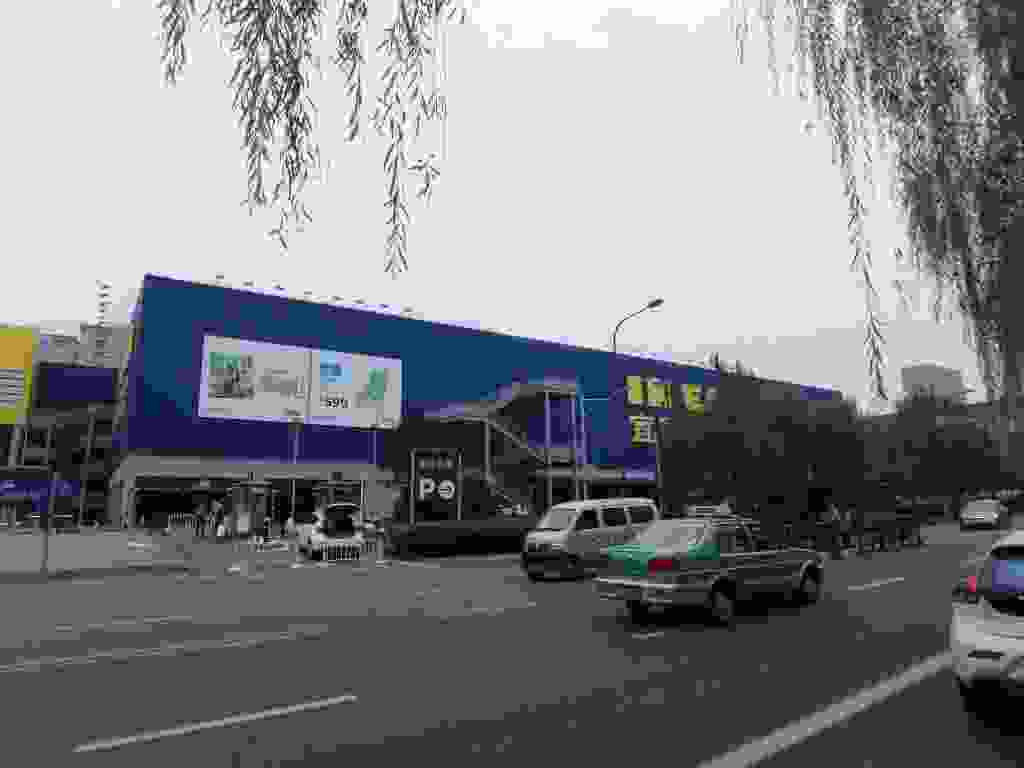
\includegraphics[width=\mywidth]{../wp-content/uploads/2015/10/wpid-p9237091-1024x768.jpg} \end{center}

\pagebreak
 Ce bâtiment est censé être le plus gros du monde. 
\begin{center} 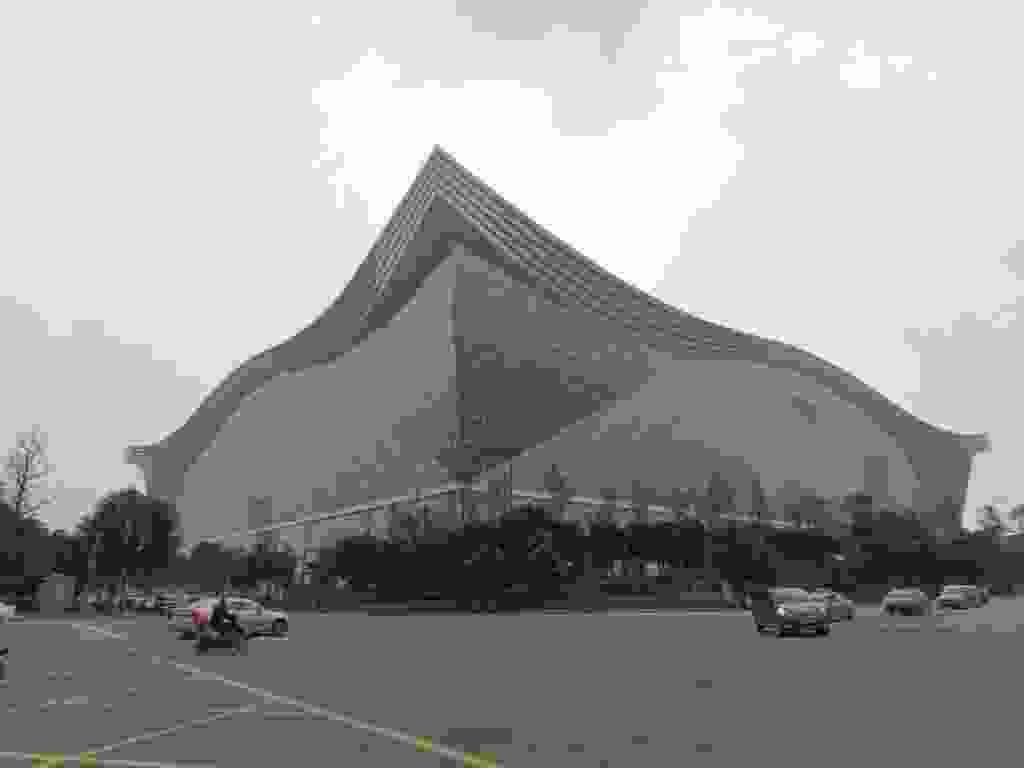
\includegraphics[width=\mywidth]{../wp-content/uploads/2015/09/wpid-p9237095-1024x768.jpg} \end{center}

 Bivouacs à 3 tentes. 
\begin{center} 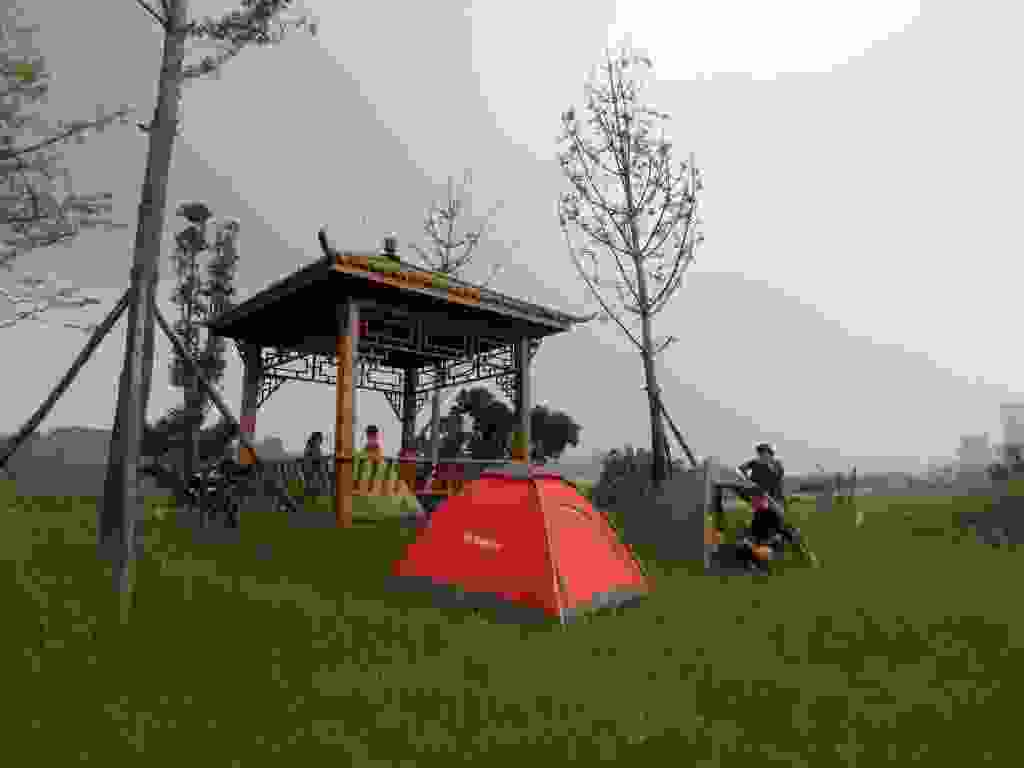
\includegraphics[width=\mywidth]{../wp-content/uploads/2015/09/wpid-p9237104-1024x768.jpg} \end{center}

\pagebreak
 Visite de Huanglongxi, petit village touristique. 
\begin{center} 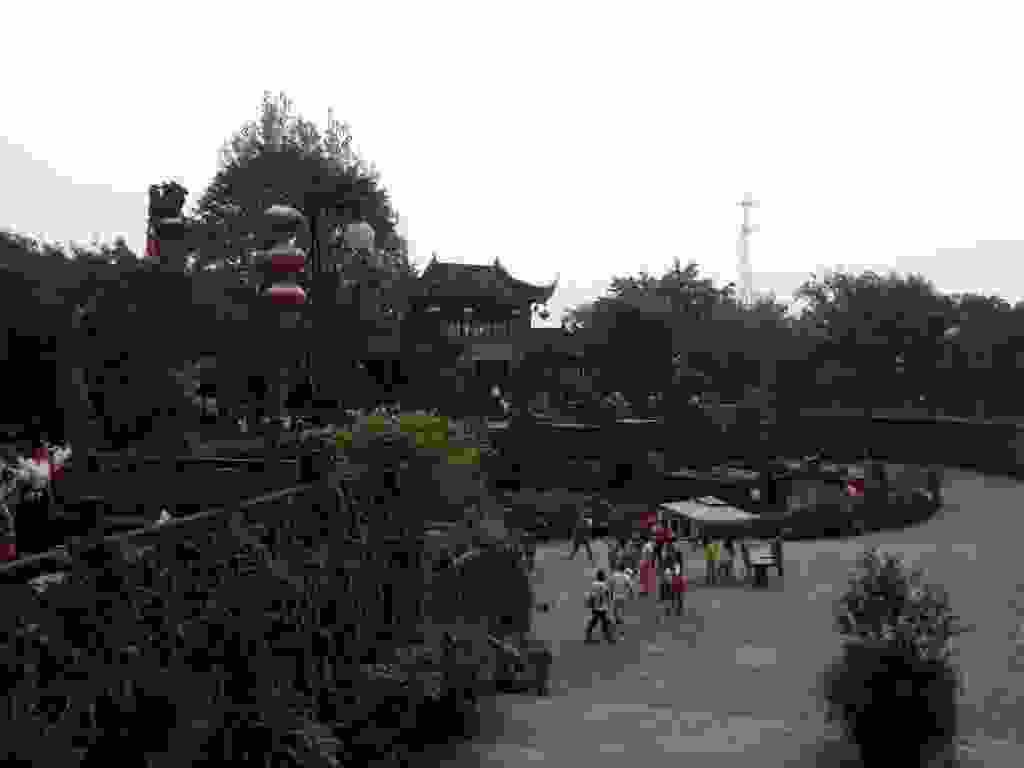
\includegraphics[width=\mywidth]{../wp-content/uploads/2015/09/wpid-p9237098-1024x768.jpg} \end{center}
\begin{center} 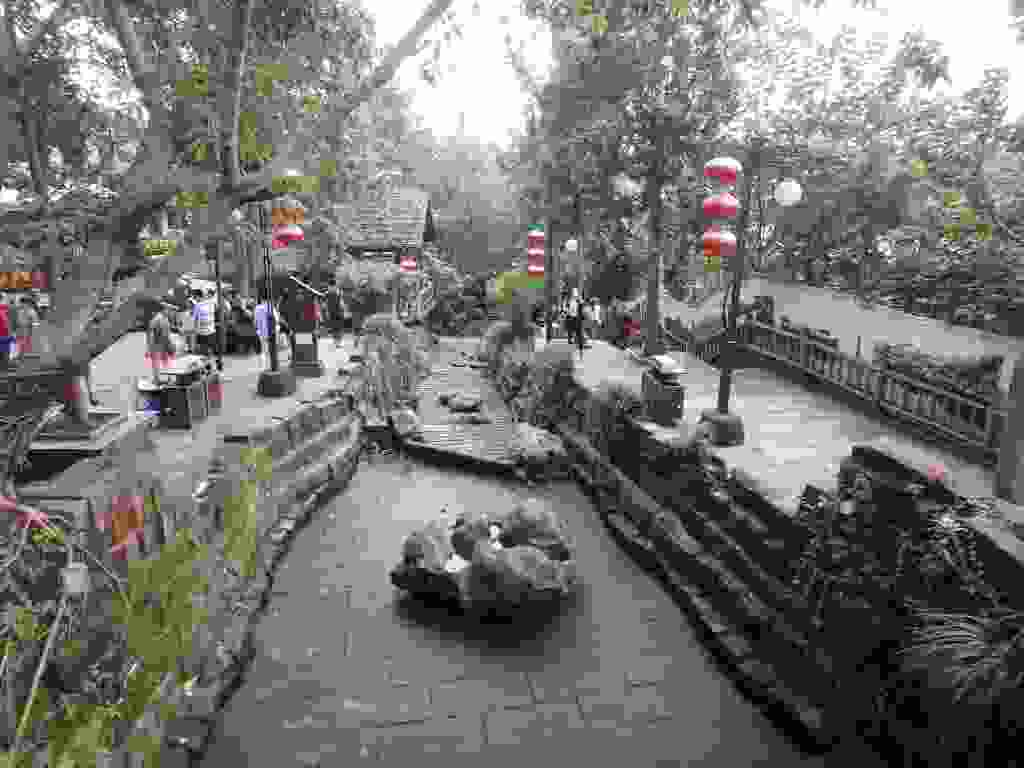
\includegraphics[width=\mywidth]{../wp-content/uploads/2015/09/wpid-p9237099-1024x768.jpg} \end{center}

\pagebreak
 Nous allons voir Emeishan, montagne sacrée du bouddhisme. Montée en bus au sommet à plus de 3000m. 
\begin{center} 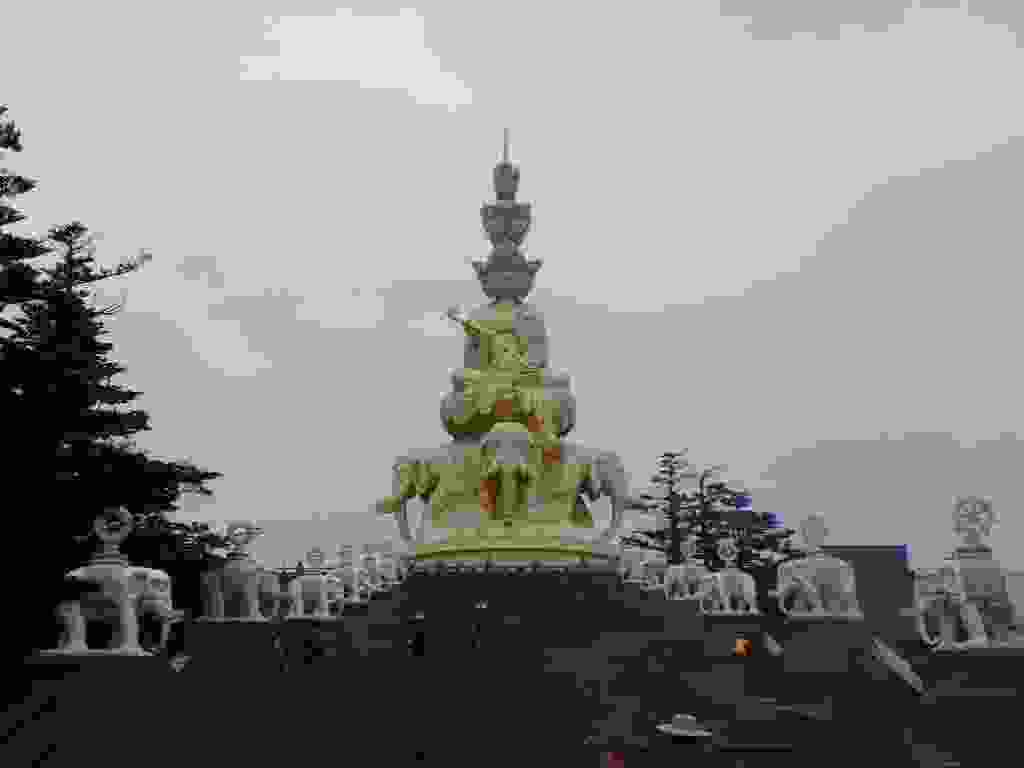
\includegraphics[width=\mywidth]{../wp-content/uploads/2015/09/wpid-p9257125-1024x768.jpg} \end{center}
\begin{center} 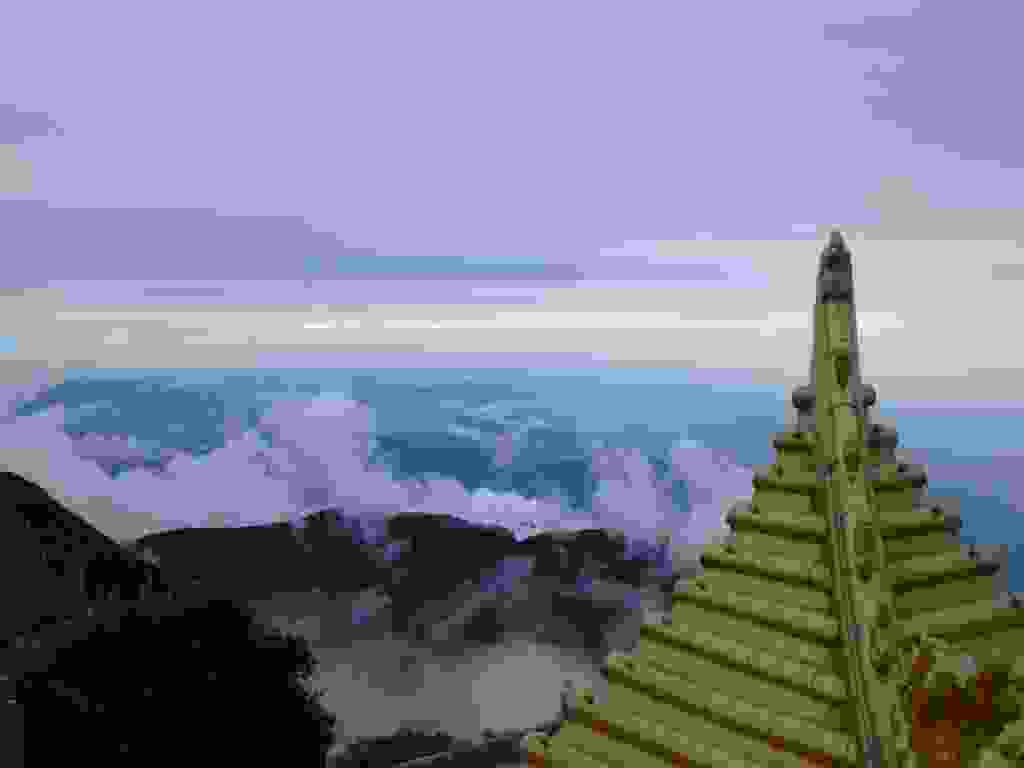
\includegraphics[width=\mywidth]{../wp-content/uploads/2015/09/wpid-p9257131-1024x768.jpg} \end{center}
\begin{center} 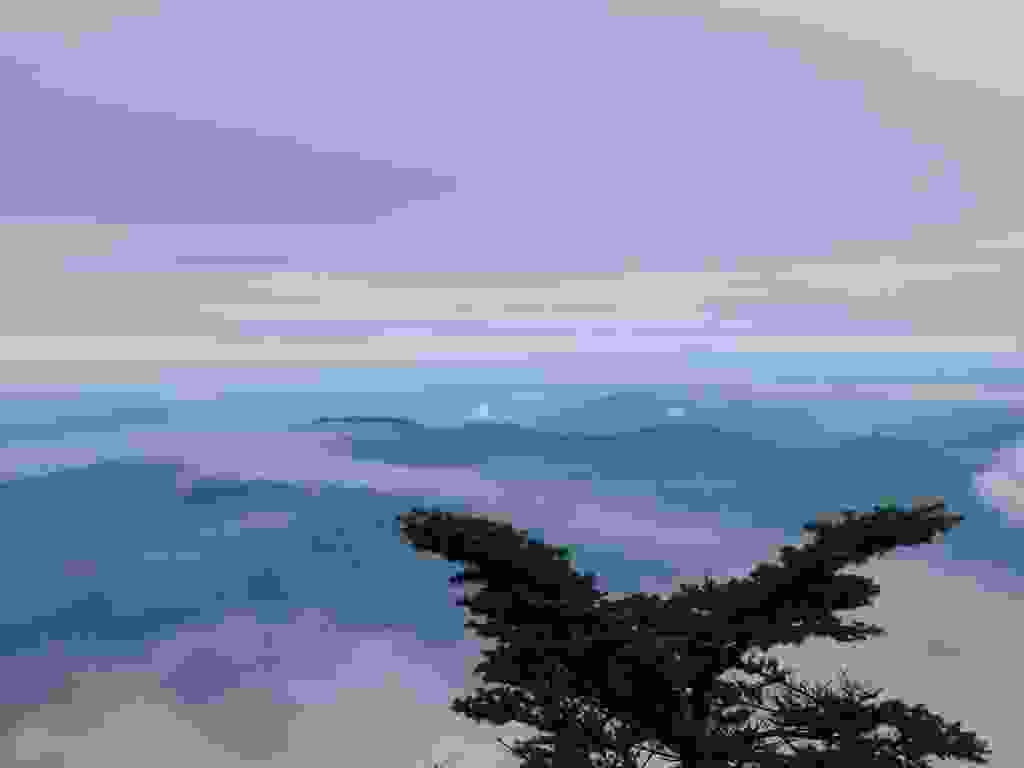
\includegraphics[width=\mywidth]{../wp-content/uploads/2015/09/wpid-p9257133-1024x768.jpg} \end{center}

 Descente à pied jusqu'en bas, que des marches : après ça impossible de prendre un escalier pendant 3 jours. 
\begin{center} 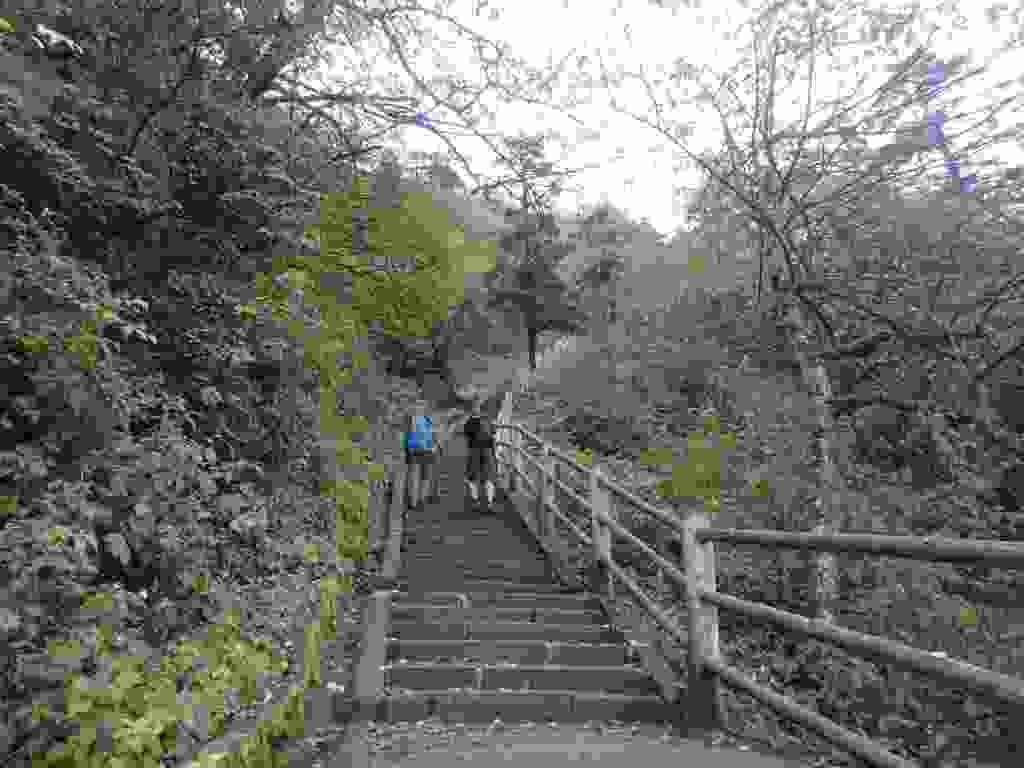
\includegraphics[width=\mywidth]{../wp-content/uploads/2015/09/wpid-p9257123-1024x768.jpg} \end{center}

\pagebreak
 Les singes sont habitués à voler la nourriture. 
\begin{center} 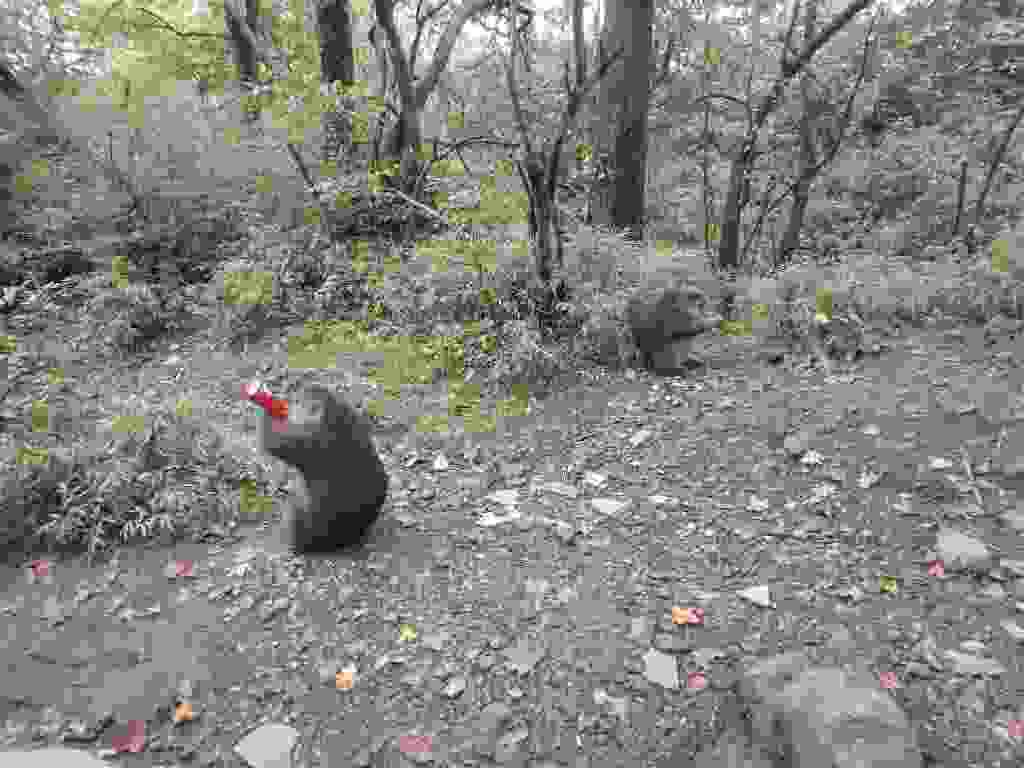
\includegraphics[width=\mywidth]{../wp-content/uploads/2015/09/wpid-p9257118-1024x768.jpg} \end{center}

 On croise régulièrement des temples sur le chemin. 
\begin{center} 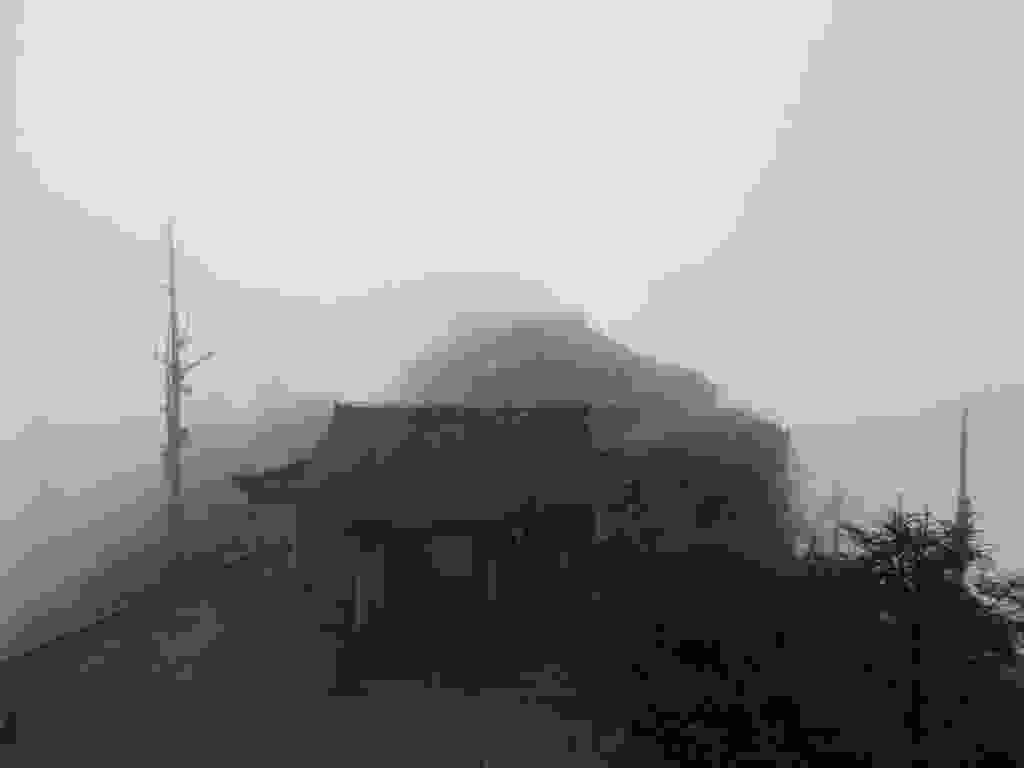
\includegraphics[width=\mywidth]{../wp-content/uploads/2015/09/wpid-p9267140-1024x768.jpg} \end{center}
\begin{center} 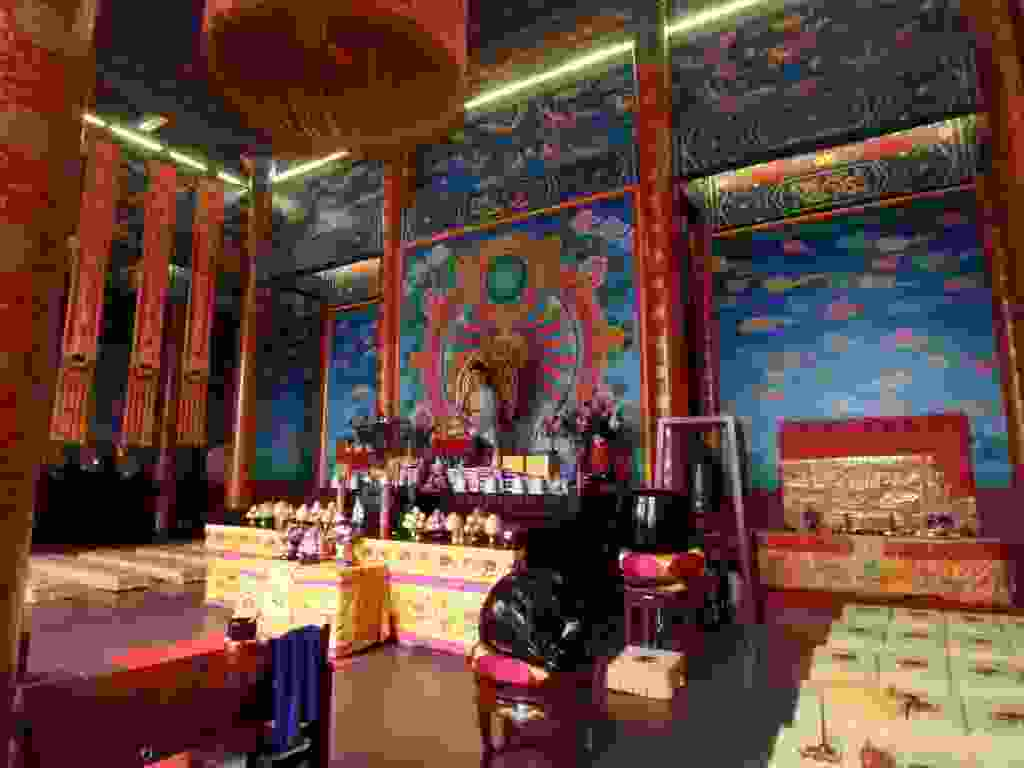
\includegraphics[width=\mywidth]{../wp-content/uploads/2015/09/wpid-p9267139-1024x768.jpg} \end{center}
\begin{center} 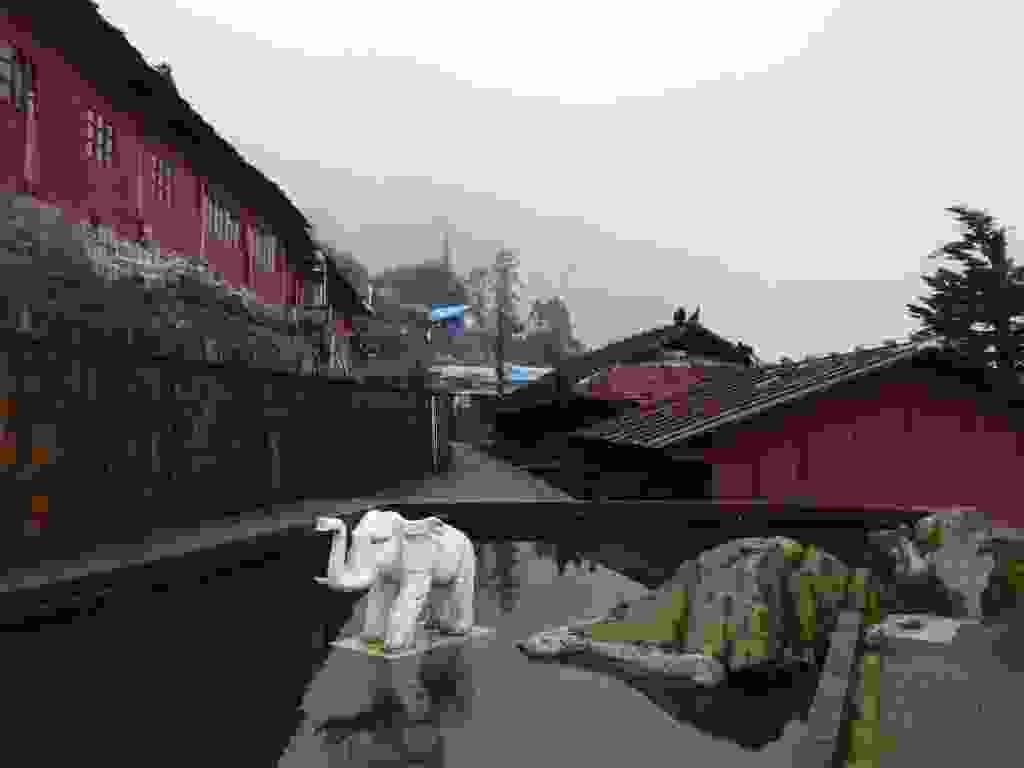
\includegraphics[width=\mywidth]{../wp-content/uploads/2015/09/wpid-p9267144-1024x768.jpg} \end{center}
\begin{center} 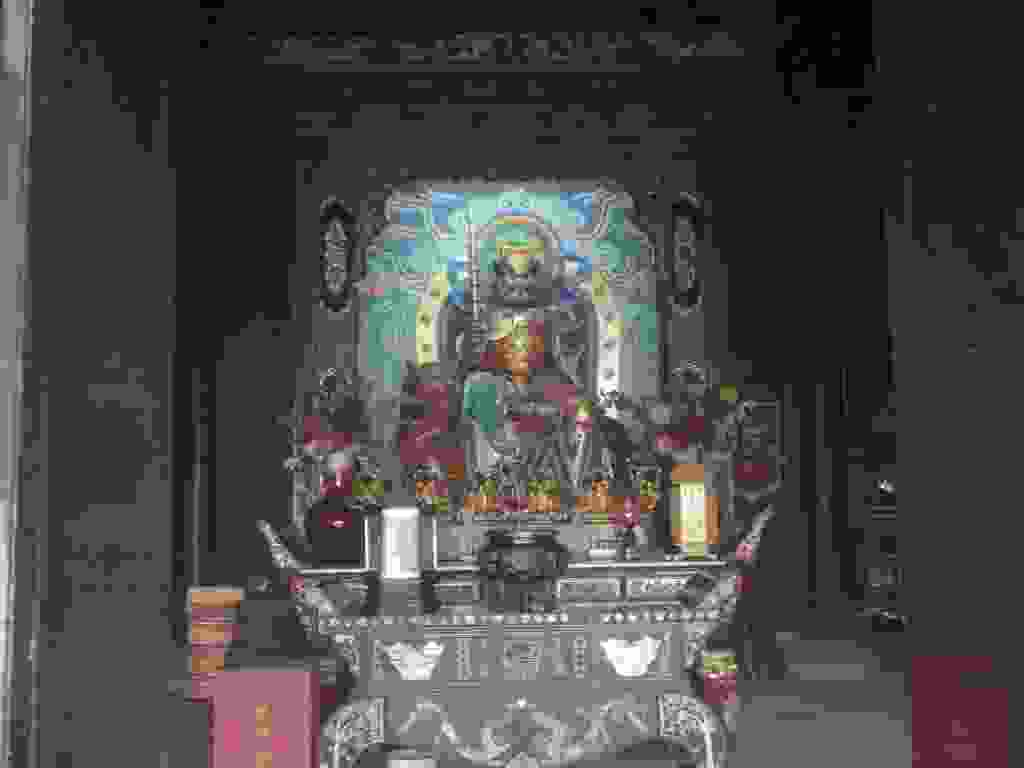
\includegraphics[width=\mywidth]{../wp-content/uploads/2015/09/wpid-p9267149-1024x768.jpg} \end{center}
\begin{center} 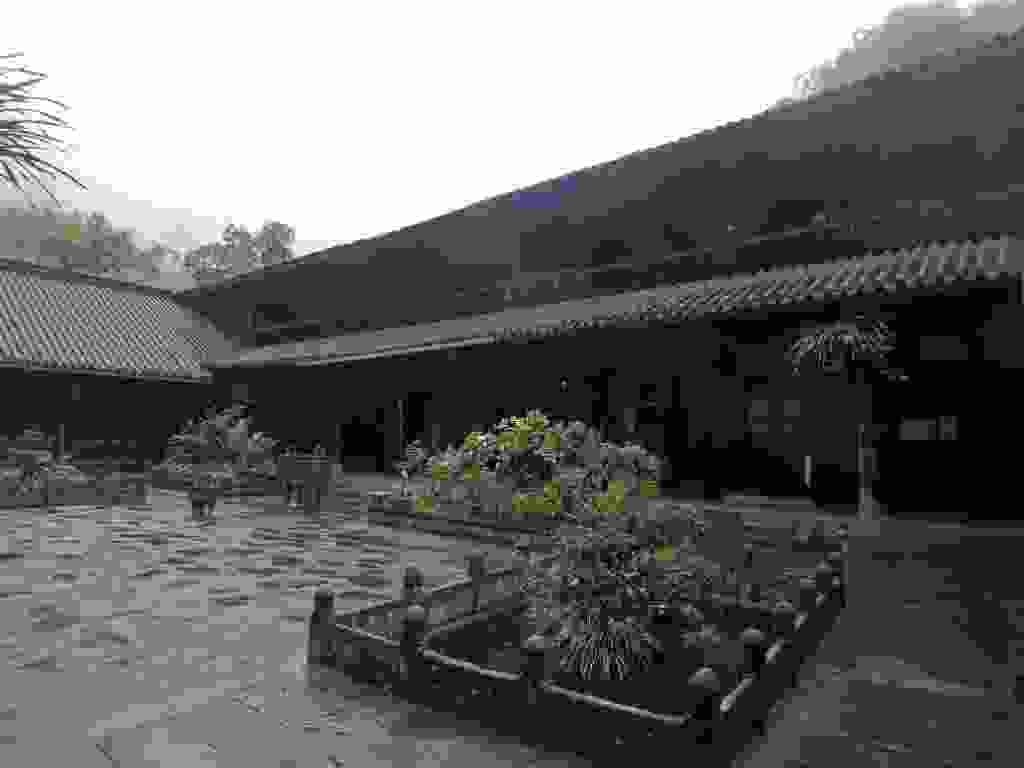
\includegraphics[width=\mywidth]{../wp-content/uploads/2015/09/wpid-p9267154-1024x768.jpg} \end{center}
\begin{center} 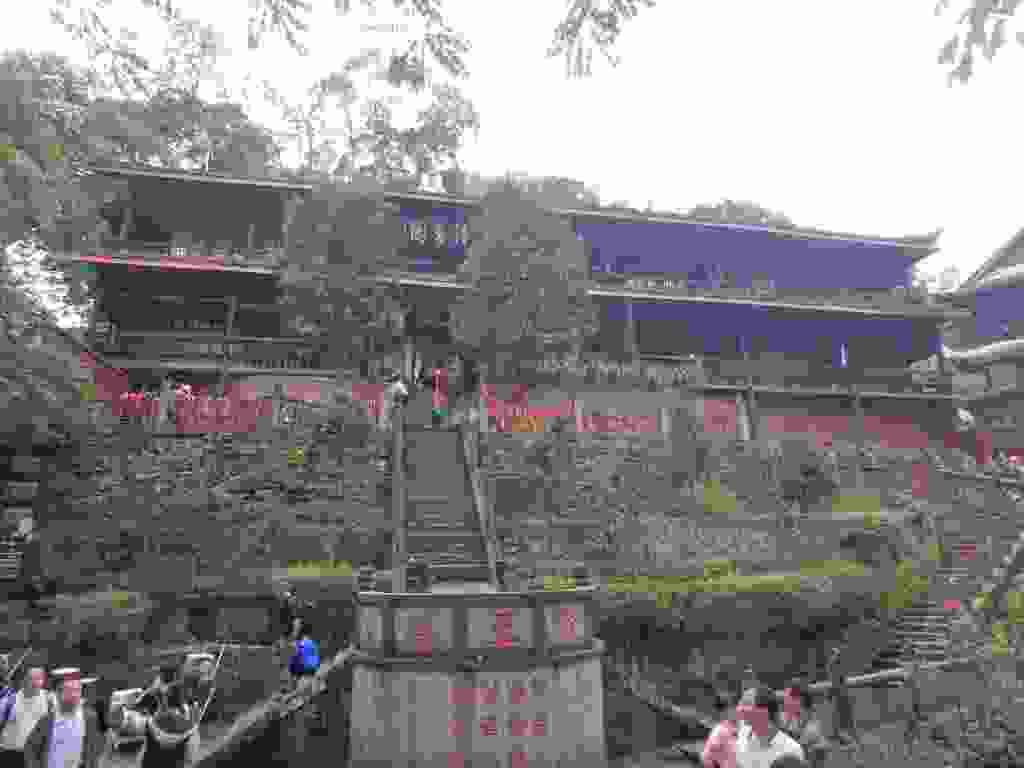
\includegraphics[width=\mywidth]{../wp-content/uploads/2015/09/wpid-p9267161-1024x768.jpg} \end{center}

 La route continue vers Leshan où je dois renouveler mon visa pour 1 mois de plus. L'occasion d'aller voir le Grand Bouddha de Leshan. 

 On passe d'abord par un temple. 
\begin{center} 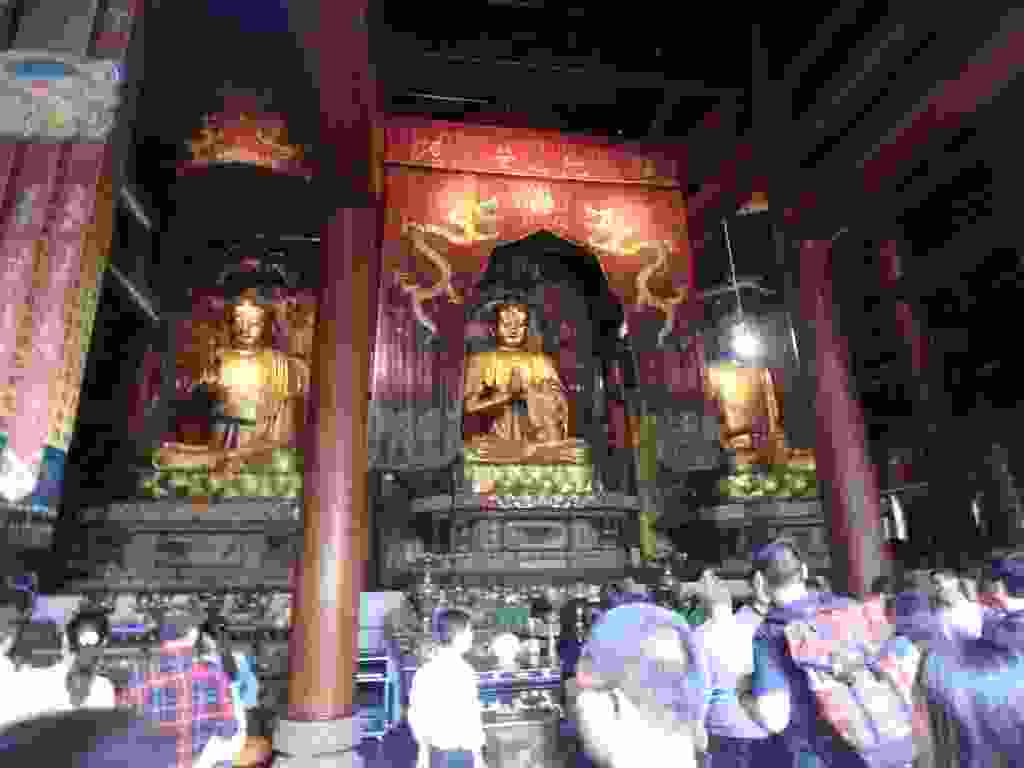
\includegraphics[width=\mywidth]{../wp-content/uploads/2015/09/wpid-p9280013-1024x768.jpg} \end{center}
\begin{center} 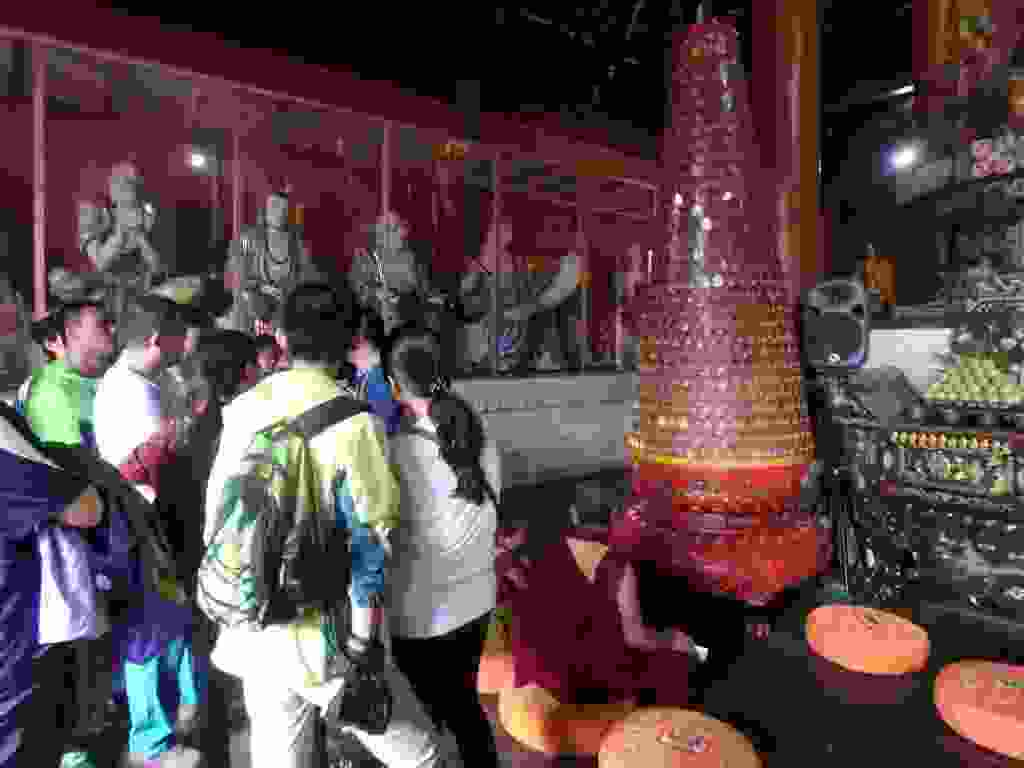
\includegraphics[width=\mywidth]{../wp-content/uploads/2015/09/wpid-p9280014-1024x768.jpg} \end{center}
\begin{center} 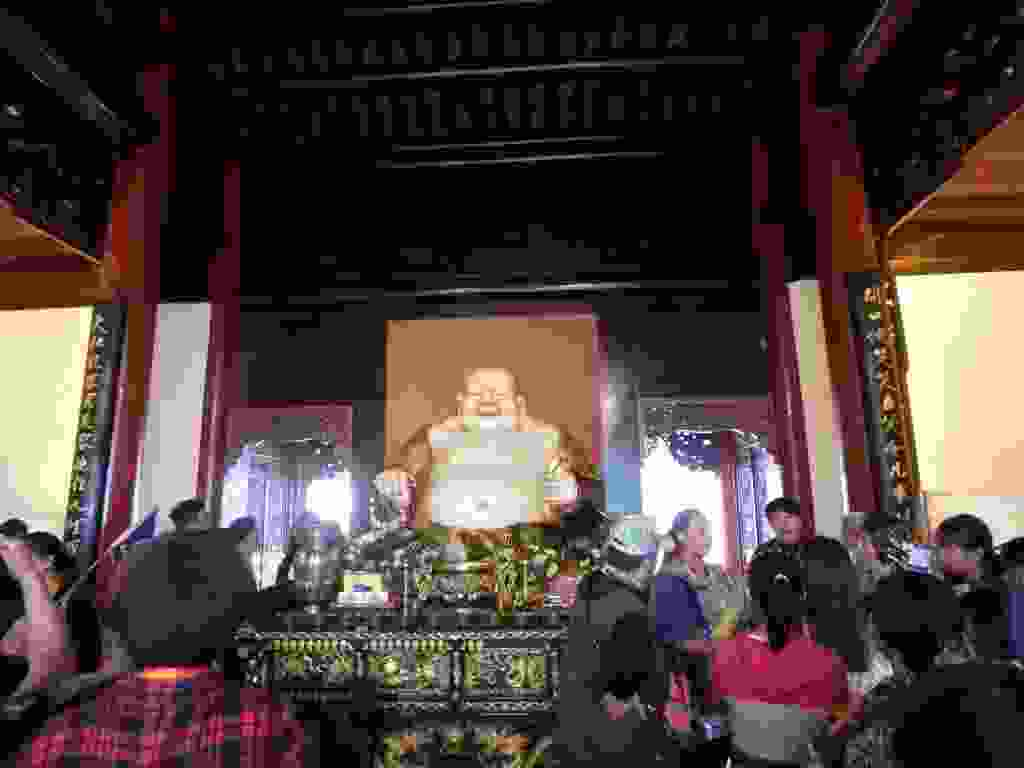
\includegraphics[width=\mywidth]{../wp-content/uploads/2015/09/wpid-p9280015-1024x768.jpg} \end{center}

\pagebreak
 Avant la descente vers le bouddha : 71m de haut. 
\begin{center} 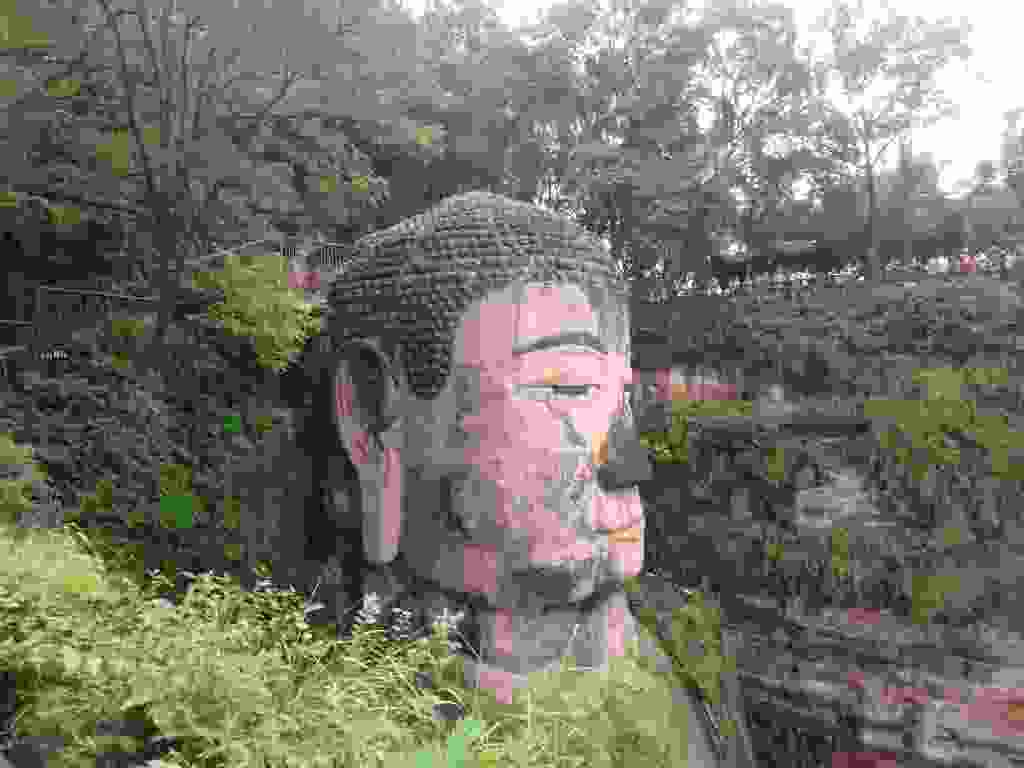
\includegraphics[width=\mywidth]{../wp-content/uploads/2015/09/wpid-p9280016-1024x768.jpg} \end{center}
\begin{center} 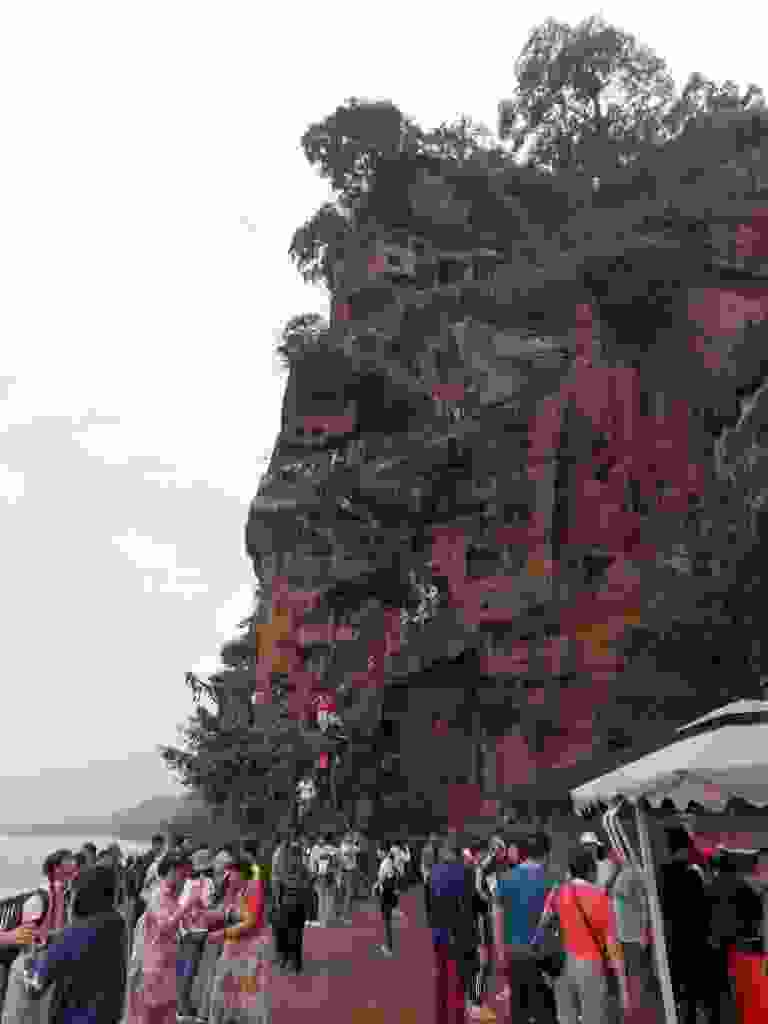
\includegraphics[height=\mywidth]{../wp-content/uploads/2015/09/wpid-p9280028-e1444295218575-768x1024.jpg} \end{center} 
\begin{center} 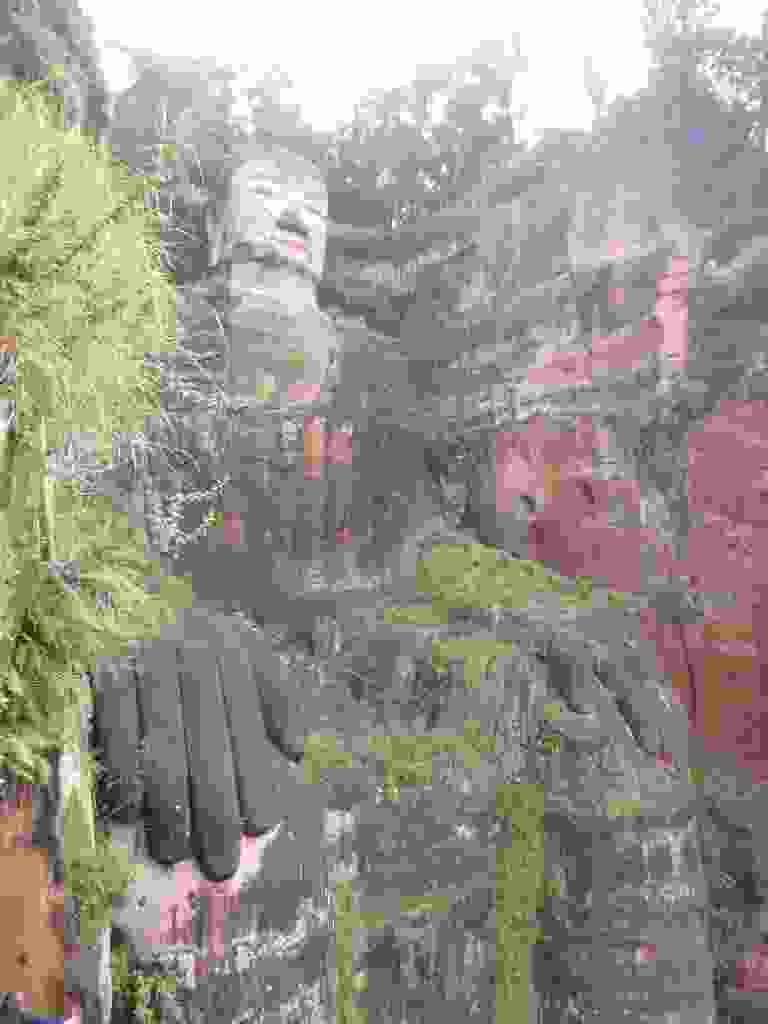
\includegraphics[height=\mywidth]{../wp-content/uploads/2015/10/wpid-p9280024-e1444295278311-768x1024.jpg} \end{center}
\begin{center} 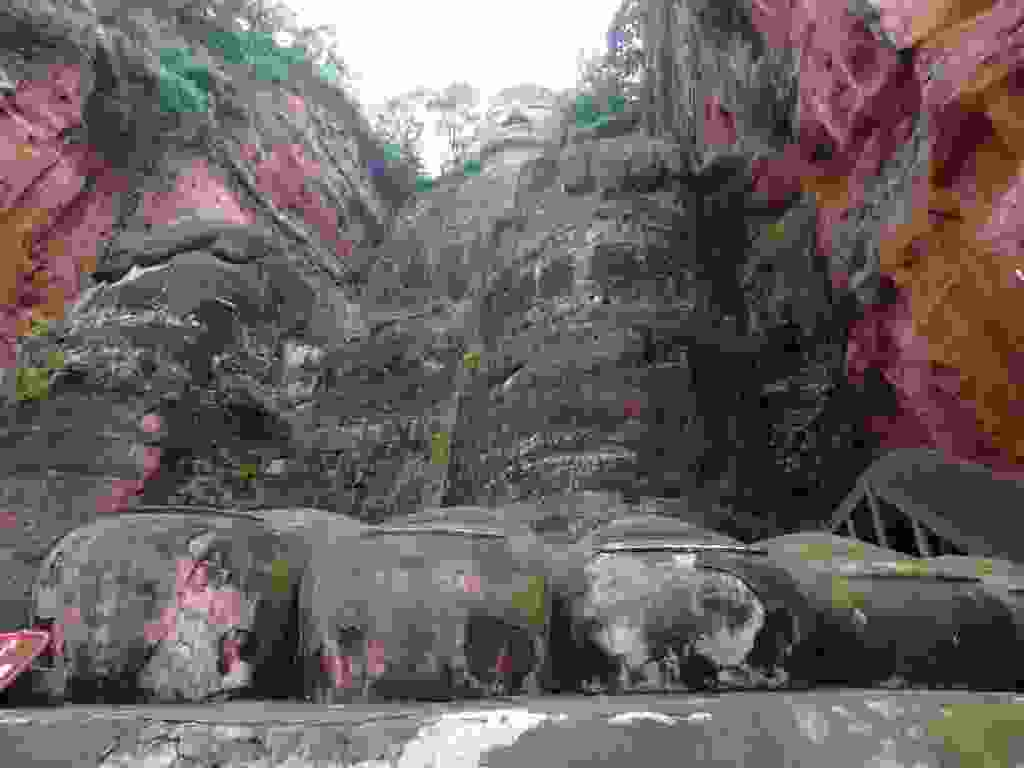
\includegraphics[width=\mywidth]{../wp-content/uploads/2015/09/wpid-p9280029-1024x768.jpg} \end{center}